\NeedsTeXFormat{LaTeX2e}
\documentclass[12pt,a4paper]{article}
\usepackage{german,a4}
\usepackage{epsfig}
\begin{document}

%%% TITLE =============================================================

\begin{titlepage}

\vspace*{\fill}
\begin{center}
\LARGE{\bf{Ein Browser f\"{u}r Alice}}
\end{center}

\vspace{1cm}

\begin{center}
  \begin{minipage}[center]{10cm}
    \begin{tabbing} 
      Bernadette Blum \hspace{1cm}\= Marvin Schiller\\
      \small{blum@ps.uni-sb.de} \> \small{schiller@ps.uni-sb.de} \\[1cm]

      Betreuer: \\[2mm]
      Thorsten Brunklaus \> Andreas Rossberg \\
      \small{brunklaus@ps.uni-sb.de} \> \small{rossberg@ps.uni-sb.de}

    \end{tabbing}
  \end{minipage}
\end{center}

\vspace{5mm}
\begin{center}
\Large{6. Mai 2003}
\end{center}

\vspace{8mm}

\begin{center}
  \begin{minipage}[center]{15cm}
    \begin{tabbing}
     Leitung: \\
     Prof. Dr. Gert Smolka \hspace{1cm}\= \small Fachbereich Informatik \\ 
    \small{smolka@ps.uni-sb.de} \> \small Universit\"{a}t des Saarlandes\\ 
    \> \small Im Stadtwald \\
    \> \small  66123 Saarbr\"{u}cken \\[5mm]
    \end{tabbing}
  \end{minipage}
\end{center}

\vspace{4mm}

%%%
%%% \begin{center}
%%%  \begin{minipage}[center]{5cm}
%%%     \small
%%%     Fachbereich Informatik\\
%%%     Universit\"{a}t des Saarlandes\\
%%%     Im Stadtwald \\
%%%     66123 Saarbr\"{u}cken \\[5mm]
%%%  \end{minipage}
%%% \end{center}


\begin{abstract}
\normalsize
Dieser Bericht zeigt Design und Implementierung eines 
interaktven Browser-Tools f\"{u}r die funktionale Programmiersprache 
Alice. Da Alice-Werte nicht selbstbeschreibend sind, 
mu\ss \, der Browser jeweils explizite Typinformationen zu denjenigen  
Werten erhalten, die dargestellt werden sollen. 
Um Werte abstrakter Typen in eine entsprechende Darstellung 
transformieren zu k\"{o}nnen, wird weiterhin 
deren Registrierung beim Browser erforderlich. 
Der Browser ist in Alice selbst implementiert und verwendet die Gtk-Bibliothek
zur Erzeugung der graphischen Benutzerschnittstele.
Unser Design kn\"{u}pft weitgehend an Thorsten Brunklaus' ''Oz Inspektor'' 
\cite{br:oz} an.
\end{abstract}

\vspace*{\fill}

\end{titlepage}

%%% EINFUEHRUNG ==========================================================

\section{Einf\"{u}hrung}  

\paragraph{}

Die graphische Aufbereitung von Programmen und Datenstrukturen erm\"{o}glicht 
Programmierern das Debuggen komplexer Programme. 
Dazu werden Algorithmen entwickelt, die man als ``Pretty Printer'' bezeichnet. 
Ziel bei der Entwicklung von Pretty Printern ist es, die Lesbarkeit eines 
Dokuments (meist Programme und mathematische Ausdr\"{u}cke) durch 
Einr\"{u}ckungen, gezielte Zeilenumbr\"{u}che und 
visuelle Atribute zu verbessern.
Dieser Bericht stellt Design und Implementierung 
eines solchen ``Pretty Printers'' f\"{u}r die Programmiersprache Alice vor. 

\paragraph{}

Die funktionale Programmiersprache Alice erm\"{o}glicht nebenl\"{a}ufige 
Programmierung und die Erzeugung zyklischer Datenstrukturen. 
Dies erlaubt es dem Programmierer, Berechnungsstr\"{a}nge (sog. Threads) 
willk\"{u}rlich zu starten oder zu beenden, Werte erst bei 
Bedarf auswerten zu lassen (sog. Laziness), oder Platzhalter 
f\"{u}r noch nicht bekannte Berechnungsergebnisse einzusetzen (sog. Futures).
\\
Die daraus resultierende Komplexit\"{a}t erfordert eine Darstellung, 
die diesen Konzepten in \"{U}bersichtlichkeit und Flexibilit\"{a}t gerecht 
wird.

\paragraph{}

Anders als beispielsweise in der Programmiersprache Oz sind 
Typen in Alice nicht selbstbeschreibend. Dadurch mu\ss \, 
zur graphischen Darstellung eines Alice-Wertes durch den 
Browser nicht nur 
der Wert selbst, sondern auch strukturelle 
Information zu diesem Wert \"{u}bergeben werden. Diese l\"{a}sst sich durch 
sogenannte Typreflektion gewinnen. Dieser Bericht zeigt auf, 
wie der Browser die strukturelle Information 
bei der Darstellung der dazugeh\"{o}rigen Werte gesteuert wird und 
welche Mechanismen n\"{o}tig sind, um Werte beliebiger abstrakter Typen 
darstellen zu k\"{o}nnen.


%%% ZENTRALE IDEEN =====================================================

\section{Zentrale Ideen}

Der Browser soll in der Lage sein, Alice-Werte 
\"ubersichtlich auf einem graphischen Interface darzustellen. 
Dies wird erreicht, indem die Werte in eine interne Beschreibung 
transformiert werden, aus der die graphische Repr\"sentation 
erzeugt werden kann. Die Transformation in 
die interne Beschreibung wird durch die 
Typinformation der inspizierten Werte gesteuert. 

\subsection{Typregistrierung}

\paragraph{}

Die Typen von Alice-Werten k\"onnen strukturelle oder abstrakte Typen 
sein. Um die Werte in eine entsprechende Darstellung transformieren 
zu k\"onnen, ben\"otigt der Browser explizite strukturelle  
Information zu diesen Werten. 

\paragraph{}

Gleichzeitig ben\"otigt der Browser Anweisungen, wie 
ein Wert eines bestimmten Types in eine interne 
Repr\"asentation und letztendlich eine graphische Darstellung 
umgewandelt werden soll.

\paragraph{}

W\"ahrend strukturelle Typen die ben\"otigte Strukturinformation 
zu dieser Transformation liefern, m\"ussen abstrakte Typen 
zusammen mit Darstellungsanweisungen beim Browser registriert 
werden. Diese Darstellungsvorschriften werden in Form einer 
Prozedur \"ubermittelt, welche die Umwandlung in eine 
Beschreibung des Wertes spezifiziert.  

\subsection{Darstellungskriterien}

\paragraph{}

Der Entwurf eines graphischen Tools erfordert die \"Uberlegung, 
welche Kriterien bei der Wahl von Anordnungsvorschriften f\"ur 
die Darstellung der Datenstrukturen im Vordergrund stehen sollen. 
Es gibt Pretty Printer, die, wie auch der 
Algorithmus von Oppen \cite{op:pr}, die Einhaltung einer vorgegebenen 
darstellbaren Seitenbreite sicherstellen, und durch gezielte 
Umbr\"uche und Einr\"uckungen die Lesbarkeit wiederherstellen. Im 
Gegensatz dazu steht die Vorgehensweise, die Anordnung nicht 
an einer vorgegebenen Seitenbreite zu orientieren, sondern 
vielmehr die Gr\"o\ss e des Darstellungsbrereichs an eine m\"oglichst 
\"ubersichtliche Darstellung anzupassen. 
Im Fall des Alice-Browsers wurde letztere Vorgehensweise gew\"ahlt, 
um trotz der Komplexit\"at der Alice-Datenstrukturen 
eine klare Darstellung zu erm\"oglichen.

\paragraph{}

Zusammengesetzte Alice-Werte lassen sich in Teilwerte untergliedern, 
so dass sich ein solcher Wert 
in eine baumartige Darstellung zerlegen l\"asst.
Hier deutet sich schon an, 
dass sich auch die interne Behandlung der Datenstrukturen 
an Baumstrukturen orientieren muss. Gleichzeitig soll der Browser 
bei der graphischen Darstellung auf 
die f\"ur Alice \"ubliche Notation f\"ur 
Werte mit Klammern und Trennzeichen 
zur\"uck greifen.    
Die Darstellung von baumartigen Werten durch 
den Browser orientiert sich dabei 
an einer Regel, wie sie u.a. Kennedy \cite{ke:dr} f\"ur 
das Baumzeichnen aufstellt: Gleiche Teilb\"aume werden 
gleich dargestellt. 

%%% Bild: Wert, interne Darstellung, graphische Darstellung

%%% ENTWURF ============================================================

\section{Entwurf}

%%% Bild: create -> layout -> draw

\subsection{Interne Darstellung}
F\"ur die interne Darstellung von Werten als B\"aume ben\"otigen wir einen 
Typen. Diesen kann man sich abstrakt als \\[2mm]
\begin{math}
doc :=  simple \\  
\hspace*{8mm} | \quad  doc_{1} \quad \hat{} \quad ... \quad \hat{} 
                \quad doc_{n} \\         
\hspace*{8mm} | \quad  
\# \lbrack doc_{1}, ... , doc_{n}\rbrack 
\\[2mm]
\end{math}
vorstellen. 

\paragraph{}

Dabei repr\"asentieren ``simples'' nur atomare Werte, die als Strings 
dargestellt werden k\"onnen. Folglich muss es sich in der Baumdarstellung 
bei ``simples'' stets um Bl\"atter eiens Baumes handeln.

\paragraph{}

Zusammengesetzte Werte bestehen im Gegensatz zu atomaren Werten aus einer
Ineinanderschachtelung von Teilwerten. Zur Darstellung solcher nicht atomaren
Werte stehen die Konkatenation \^\quad und die Akkumulation 
\# \lbrack \, \rbrack \quad zur Verf\"ugung.
W\"ahrend die Konkatenation stets horizontal anordnet (vergleichbar mit der 
sogenannten ``hbox'' bei manchen Pretty Printern), 
erfolgt bei der Akkumulation in der Aufbauphase 
noch keine Entscheidung, ob die Kindknoten eines Knotens horizontal oder 
vertikal dargestellt werden. Diese Entscheidung wird erst beim Layoutvorgang
getroffen (n\"ahere Erl\"auterung dazu siehe 4.4).

\paragraph{}

Der Wert \large{(1, 2)} \normalsize wird in die folgende interne 
baumartige Darstellung transformiert: \\


\begin{center}
\epsfig{file = ex_tree_bw.ps, width = 13cm}
\linebreak Abbildung 4.1: Beispiel f\"ur interne Darstellung
\end{center}

\subsection{Typregistrierung}

\subsection{Transientenverwaltung}

\paragraph{}

Transienten, die in Alice als Byneeds (bei der sogenannten ``Laziness''), 
Promises oder Futures auftreten k\"onnen, werden in der Browserdarstellung
als solche gekennzeichnet. Sobald sie zu einem Wert auswerten, muss
die Darstellung des Browsers aktualisiert werden. Deshalb wird
f\"ur jeden Transienten ein W\"achter ben\"otigt, der diesen \"uberwacht.
Nimmt ein Transient, der in mehreren bereits dargestellten 
Datenstrukturen bzw. mehrmals in der gleichen Datenstruktur auftritt, 
einen konkreten Wert an, so l\"ost sein W\"achter einen Updatemechanismus 
aus, der alle seine Auftreten durch diesen Wert ersetzt.
Folglich muss jeder W\"achter den Transienten kennen, den er \"uberwacht, 
und zus\"atzlich alle Knoten, die diesen Transienten repr\"asentieren. 

\begin{center}
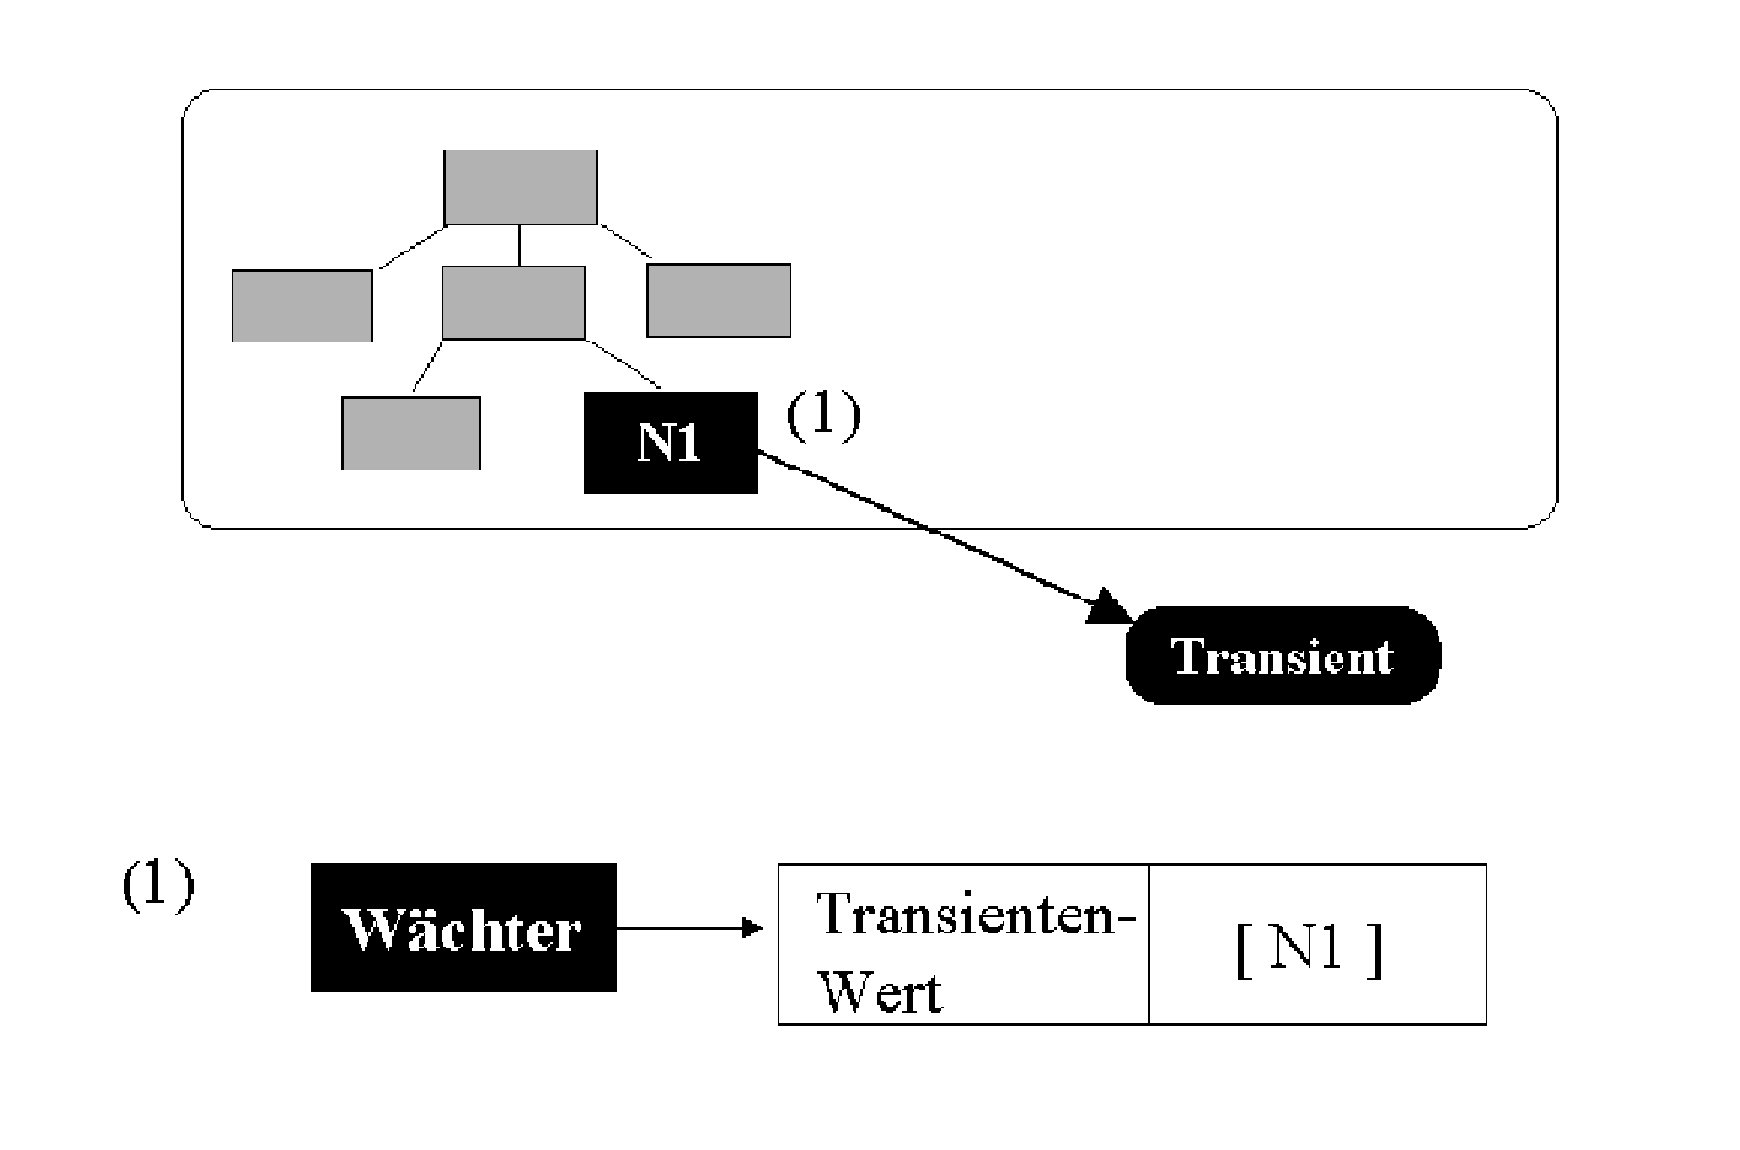
\epsfig{file = transient1_bw.ps, width = 12cm}
\linebreak 
Abbildung 3.1: Transient mit W\"{a}chter
\end{center}

\subsection{Graphmodus}

\subsection{Filter} 


%%% IMPLEMENTIERUNG ====================================================

\section{Implementierung}

\subsection{Knotentypen}

\subsection{Typregistrierung und -zerlegung}

\subsection{Layout}

\subsection{Zeichnen}

\subsection{Inkrementalit\"at} 


\subsection{Transientenverwaltung}

\subsection{Module}

\begin{center}
\epsfig{file = module_bw.ps, width = 13cm}
\linebreak Abbildung 4.6: Module des Browsers
\end{center}

Abbildung 4.6 zeigt die Module des Browsers. 
Diese lassen sich nach ihrer Funktionalit\"at gruppieren.
\newline
Die Basismodule Doc und Node enthalten die Datentypen
der internen Beschreibung - doc und node - und die
entsprechenden Accessoren. Da diese w\"{a}hrend der 
Erzeugnung, der Anordnungsberechnung, des Zeichnens 
und der Darstellungsaktualisierung verwendet werden, 
werden sie von vielen anderen Modulen benutzt. Zur Gruppe 
der Basismodule z\"ahlt auch das Modul GtkSupport, das die
Gtk-Funktionalit\"at gegen\"uber allen anderen Modulen des 
Browsers abkapselt. Als einziges Modul hat es direkten Zugriff 
auf die Gtk-Prozeduren, alle anderen Module greifen auf 
GtkSupport zur\"uck. \newline \hspace*{5mm}
Zur zweiten Gruppe geh\"oren die Module CreateTree, Layout, Draw 
und Update. CreateTree, Layout, und Draw repr\"{a}sentieren 
die drei Phasen des Inspektionsvorgangs, w\"ahrend  Update die 
notwendigen Mechanismen zur Aktualisierung der Darstellung
enth\"alt. \newline \hspace*{5mm}
Mithilfe der Module Widget und UnsafeInspector wird die 
Benutzerschnittstelle erzeugt. Widget verf\"ugt \"uber die 
graphische Benutzeroberfl\"ache und steuert die 
Darstellungserzeugung bzw. -ver\"anderung. UnsafeInspector macht 
die f\"ur den Benutzer relevanten Prozeduren und Datentypen nach 
au\ss en sichtbar. \newline \hspace*{5mm}
Alle Aktionen des Browsers \"uber den Server synchronisiert.


%%% AUSBLICK ===========================================================

\section{Ausblick}

Zur Zeit verwenden wir ein Gtk-Binding f\"ur Mozart \cite{mo:mo}
zur Erzeugung der graphischen Benutzeroberfl\"ache. Allerdings ist 
es auch m\"oglich, den Browser an eine von Robert Grabowski im Rahmen 
seines Fortgeschrittenenpraktikums neu implementierte Gtk-Schnittstelle
f\"ur Alice \cite{gr:gt} anzuschlie\ss en.

\paragraph{}

Desweiteren ist der Alice-Browser nicht typsicher, 
da der Benutzer zur Zeit ein Tupel aus 
Wert und mithilfe des Typreflektors reflektierten Typs 
an die inspect-Funktion \"ubergibt.  
Eine automatische Typreflektion w\"urde die Benutzung des Tools 
erleichtern und eine Fehlbenutzung ausschlie\ss en. 
In diesem Fall m\"usste der Benutzer nur noch den zu 
inspizierenden Wert \"ubergeben. 

Mithilfe eines \"ubergeordneten Funktors lie\ss e 
sich der Browser einkapseln.

%%% BIBLIOGRAPHIE =======================================================

\begin{thebibliography}{99}

\bibitem{br:oz} Thorsten Brunklaus 2000. {\em Der Oz Inspector - Browsen: 
    Interaktiver, einfacher, effizienter} Diplomarbeit, Universit\"{a}t 
    des Saarlandes, Fachbereich Informatik.
\bibitem{op:pr} Derek Oppen 1980.{\em Prettyprinting} ACM Transactions 
  on Programming Languages and Systems, Bd. 2, Nr.4, 1980, pp 465-483.
\bibitem{ke:dr} Andrew Kennedy 1996. {\em Drawing Trees} 
                Journal of Functional Programming, Bd. 6(3), pp. 527-534.
\bibitem{al:al} Alice-Homepage: www.ps.uni-sb.de/alice/
\bibitem{gt:gt} GTK+: The Gimp Toolkit: www.gtk.org 
\bibitem{mo:mo} The Mozart Programming System: www.mozart-oz.org/
\bibitem{gr:gt} Robert Grabowski 2003. {\em Eine Gtk-Schnittstelle f\"ur 
                Alice} 
                FoPra-Ausarbeitung, Lehrstuhl Prof. G. Smolka, 
                Universtit\"at des Saarlandes.

\end{thebibliography}

\end{document}

